


% \vspace{-0.05cm}
% \subsection{}
% \vspace{-0.05cm}

\begin{figure}[t]
    \centering
    \hspace*{-0.5cm}    
    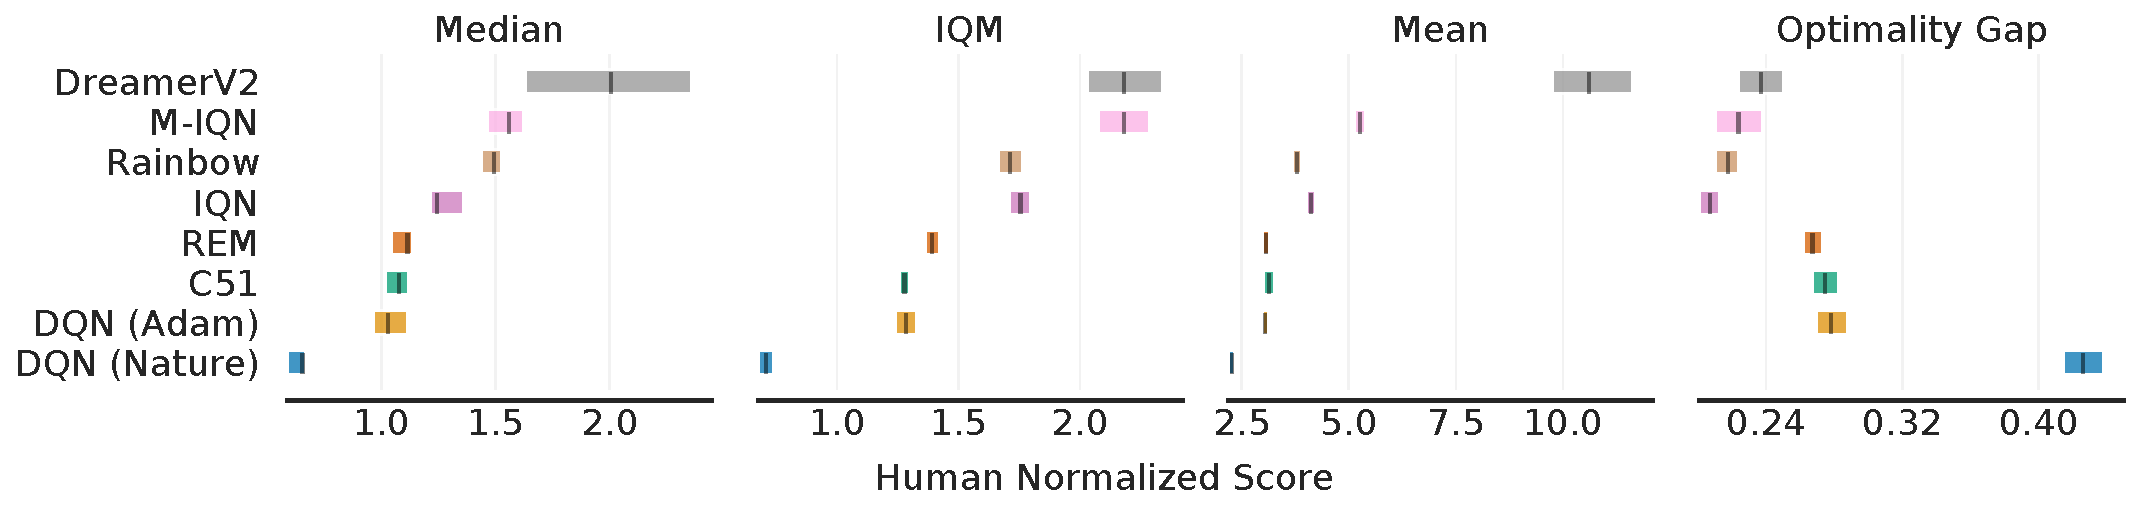
\includegraphics[width=\linewidth]{new_figures/atari_aggregates.pdf}
    \vspace{-0.1cm}
    \caption{\textbf{Aggregate metrics on Atari 200M} with 95\% CIs based on 55 games with sticky actions~\citep{machado2018revisiting}. Higher mean, median and IQM scores and lower optimality gap are better. The CIs are estimated using the percentile bootstrap with stratified sampling. IQM typically results in smaller CIs than median scores. Large values of mean scores relative to median and IQM indicate being dominated by a few high performing tasks, for example, DreamerV2 and M-IQN obtain normalized scores above 50 on the game \textsc{JamesBond}. Optimality gap is less susceptible to outliers compared to mean scores. We compare DQN~(Nature)~\citep{mnih2015human}, DQN with Adam optimizer, C51~\citep{bellemare2017distributional}, REM~\citep{agarwal2020optimistic}, Rainbow~\citep{hessel2018rainbow},
    IQN~\citep{dabney2018implicit}, Munchausen-IQN~(M-IQN)~\citep{vieillard2020munchausen}, and DreamerV2~\citep{hafner2020mastering}. All results are based on 5 runs per game except for M-IQN and DreamerV2 which report results with 3 and 11 runs.}
    \label{fig:atari_aggregates}
    % \vspace{-0.25cm}
    \vspace{-0.4cm}
\end{figure}



\textbf{Arcade Learning Environment}. Training RL agents for 200M frames on the ALE~\citep{bellemare2013arcade, machado2018revisiting} is the most widely recognized benchmark in deep RL. We revisit some popular methods which demonstrated progress on this benchmark and reveal discrepancies in their findings as a consequence of ignoring the uncertainty in their results~(\figref{fig:atari_aggregates}). For example, DreamerV2~\citep{hafner2020mastering} exhibits a large amount of uncertainty in aggregate scores. While M-IQN~\citep{vieillard2020munchausen} claimed better performance than Dopamine Rainbow\footnote{Dopamine Rainbow differs from that of \citet{hessel2018rainbow} by not including double DQN, dueling architecture and noisy networks. Also, results in \citep{hessel2018rainbow} were reported using a single run without sticky actions.}~\citep{hessel2018rainbow} in terms of median normalized scores, their interval estimates strikingly overlap. Similarly, while C51~\citep{bellemare2013arcade} is considered substantially better than DQN~\citep{mnih2015human}, the interval estimates as well as performance profiles for DQN~(Adam) and C51 overlap significantly. 

\figref{fig:atari_aggregates} reveals an interesting limitation of aggregate metrics: depending on the choice of metric, the ordering between algorithms changes~(\eg Median \versus IQM). The inconsistency in ranking across aggregate metrics arises from the fact that such metrics only capture a specific aspect of overall performance across tasks and runs. Additionally, the change of algorithm ranking between optimality gap and IQM/median scores reveal that while recent algorithms typically show performance gains relative to humans on average, their performance seems to be worse on games below human performance. Since performance profiles capture the full picture, they would often illustrate why such inconsistencies exist. For example, optimality gap and IQM can be both read as areas in the profile~(\figref{fig:aggregate_metrics}). The performance profile in \figref{fig:perfProfilesAtari200M}~(left) illustrates the nuances present when comparing different algorithms. For example,  IQN seems to be better than Rainbow for $\tau \geq 2$, but worse for $\tau < 2$. Similarly, the profiles of DreamerV2 and M-IQN for $\tau < 8$  intersect at multiple points. To compare sample efficiency of the agents, we also present their IQM scores as a function of number of frames in \figref{fig:perfProfilesAtari200M}~(right). 

%This plot shows that gains from C51 and REM over DQN~(Adam) were relatively small, while gains from DreamerV2 and M-IQN have high uncertainty.

% \textbf{Remark}. .

\begin{figure}[t]
    \centering
    % \includegraphics[width=0.47\linewidth]{figures/atari_200m_perf.pdf}
    
\includegraphics[width=0.96\linewidth]{new_figures/atari_200m_legend.pdf}
    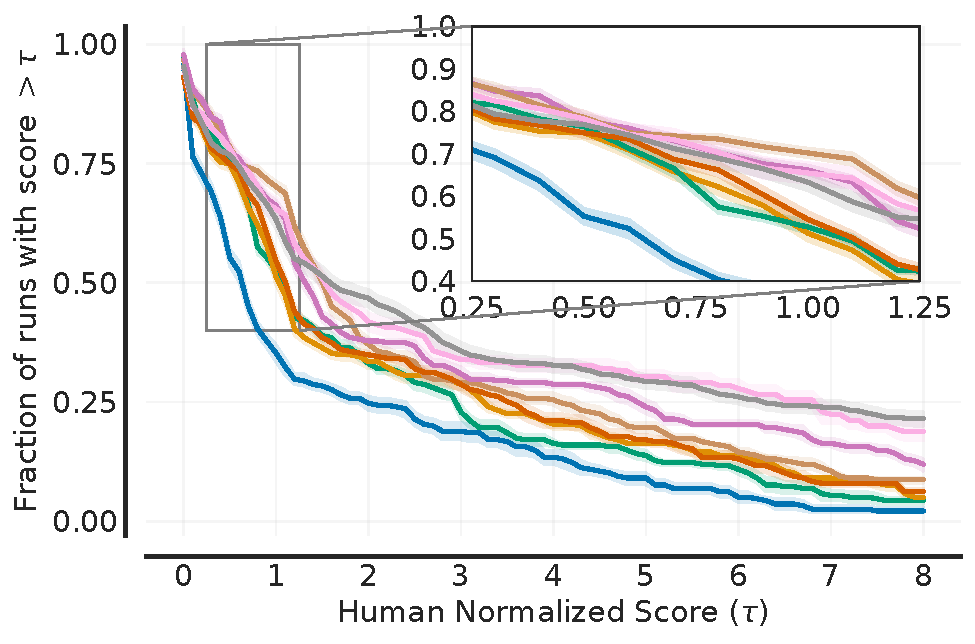
\includegraphics[width=0.47\linewidth]{new_figures/atari_200m_perf_inset.pdf}
    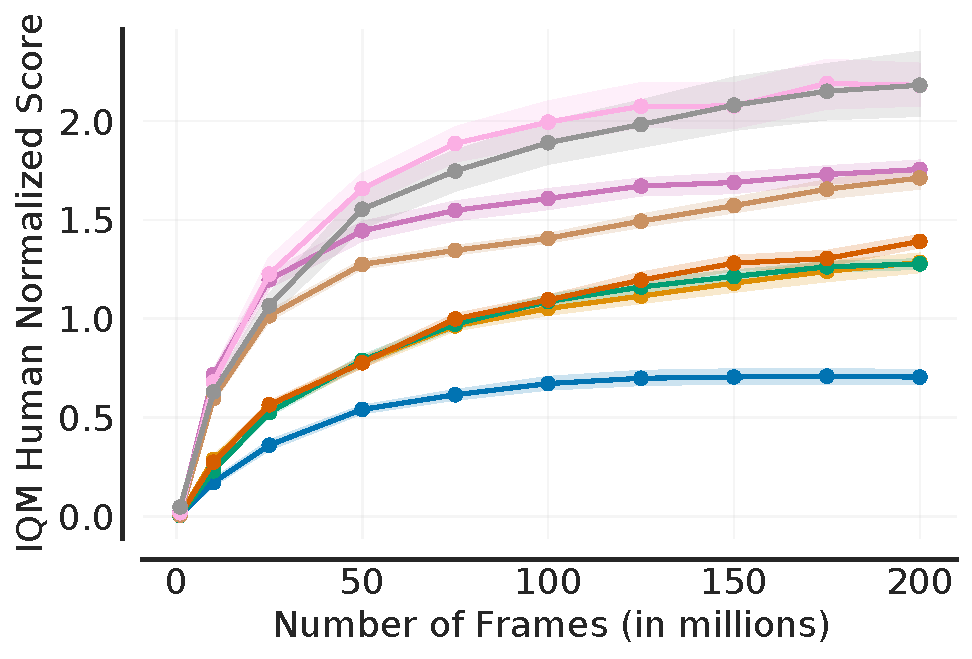
\includegraphics[width=0.47\linewidth]{new_figures/atari_sample_efficiency_iqm.pdf}
    \vspace{-0.1cm}
    \caption{\textbf{Atari 200M evaluation}. \textbf{Left}. Score distributions using human-normalized scores obtained after training for 200M frames. \textbf{Right}. Sample-efficiency of agents as a function of number of frames measured via IQM human-normalized scores. Shaded regions show pointwise 95\% percentile stratified bootstrap CIs.}\label{fig:perfProfilesAtari200M}
    % \vspace{-0.2cm}
\end{figure}



% On the other hand, the tail end of the distributions ($\tau > 8$) suggests a clear ordering of DreamerV2, M-IQN, and the rest. However, as the optimality gap plot in \figref{fig:atari_aggregates} demonstrates, this tail-end may be over-emphasizing games for which RL agents can already perform at levels far superior to that of an average human player.



\begin{figure}[t]
    \centering
    \begin{subfigure}[l]{0.47\textwidth}
        \centering
        \vspace{-0.1cm}
        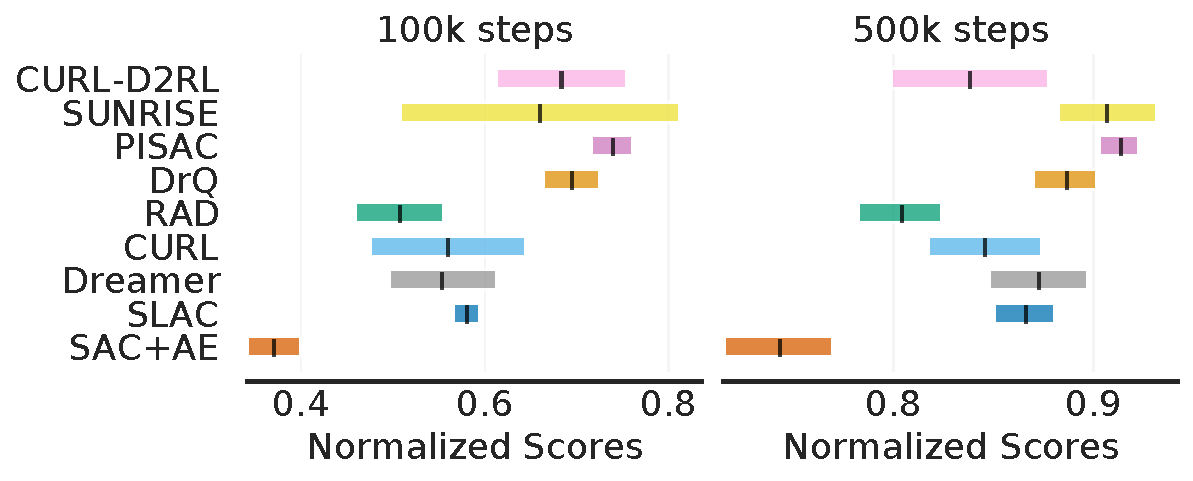
\includegraphics[width=\textwidth]{new_figures/dmc_mean_scores.pdf}
        \vspace{-0.3cm}
        \caption{\small Mean Scores ($=1$ - Optimality Gap)}\label{res:dm_control_mean}
    \end{subfigure}
    \begin{subfigure}[l]{0.28\textwidth}
        \centering
        \vspace{-0.4cm}
        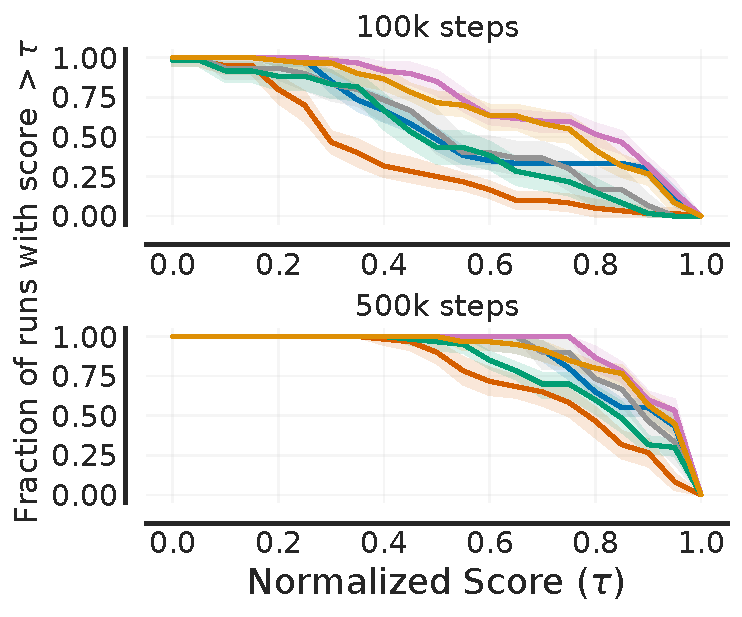
\includegraphics[width=\textwidth]{new_figures/dmc_perf_profile.pdf}
        \vspace{-0.6cm}
        \caption{\small Score Distributions.}\label{res:dm_control_profiles}
    \end{subfigure}
    \begin{subfigure}[l]{0.23\textwidth}
        \centering
        \vspace{-0.4cm}
        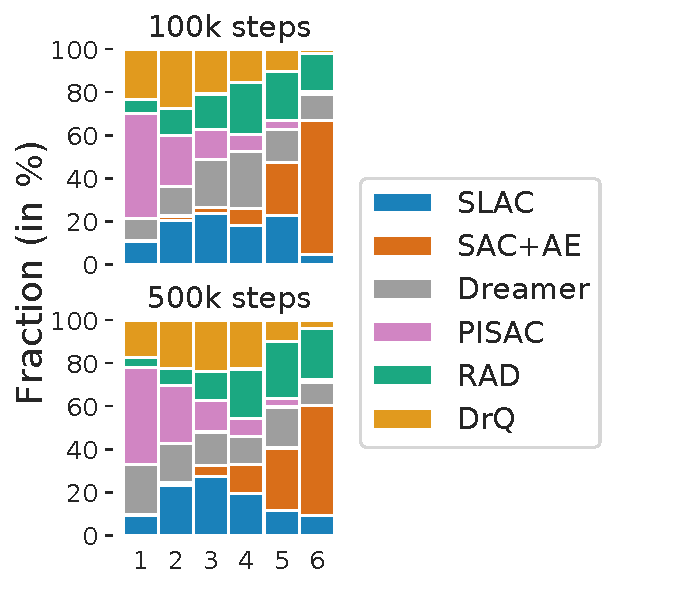
\includegraphics[width=\textwidth]{new_figures/dmc_ranking_vertical.pdf}
        \vspace{-0.3cm}
        \caption{\small Rank comparisons.}\label{res:dm_control_rank}
    \end{subfigure}
    \vspace{-0.1cm}
    \caption{\textbf{DeepMind Control Suite evaluation} results, averaged across 6 tasks, on the 100k and 500k benchmark. We compare SAC+AE~\citep{yarats2019improving}, SLAC~\citep{lee2020stochastic}, Dreamer~\citep{hafner2019dream}, CURL~\citep{srinivas2020curlv2}, RAD~\citep{laskin2020reinforcement}, DrQ~\citep{yarats2021image}, PISAC~\citep{lee2020predictive},
    SUNRISE~\citep{lee2020sunrise}, and CURL-D2RL~\citep{sinha2020d2rl}. The \textbf{ordering} of the algorithms in the left figure is based on their claimed relative performance -- all algorithms except Dreamer claimed improvement over at least one algorithm placed below them. %Individual runs for each method were  except for  for which we used their reported scores.
    % for which their authors were not able to provide individual runs. 
    \textbf{(a)} Interval estimates show 95\% stratified bootstrap CIs for methods with individual runs provided by their respective authors and 95\% studentized CIs for CURL, CURL-D2RL, and SUNRISE. Normalized scores are computed by dividing by the maximum score~(=1000). \textbf{(b)} Score distributions. \textbf{(c)} The $i^{th}$ column in the rank distribution plots show the probability that a given method is assigned rank $i$, averaged across all tasks.  The ranks are estimated using 200,000 stratified bootstrap re-samples.}\label{res:dm_control}
    \vspace{-0.45cm}
\end{figure}


% \vspace{-0.25cm}
% \subsection{}
% \vspace{-0.25cm}
\textbf{DeepMind Control Suite}. Recent continuous control papers benchmark performance on 6 tasks in DM Control~\citep{tassa2018deepmind} at 100k and 500k steps. Typically, such papers claim improvement based on higher mean scores per task regardless of the variability in those scores. However, we find that when accounting for uncertainty in results, most algorithms do not consistently rank above algorithms they claimed to improve upon~(\figref{res:dm_control_rank} and \ref{res:dm_control_profiles}). Furthermore, there are huge overlaps in 95\% CIs of mean normalized scores for most algorithms~(\figref{res:dm_control_mean}). These findings suggest that a lot of the reported improvements are spurious, resulting from randomness in the experimental protocol.




% \vspace{-0.25cm}
%  benchmark}
% \vspace{-0.15cm}

\begin{figure}[t]
    \centering
    % \begin{subfigure}[c]{0.49\textwidth}
        % \centering
        % \vspace{-0.05cm}
        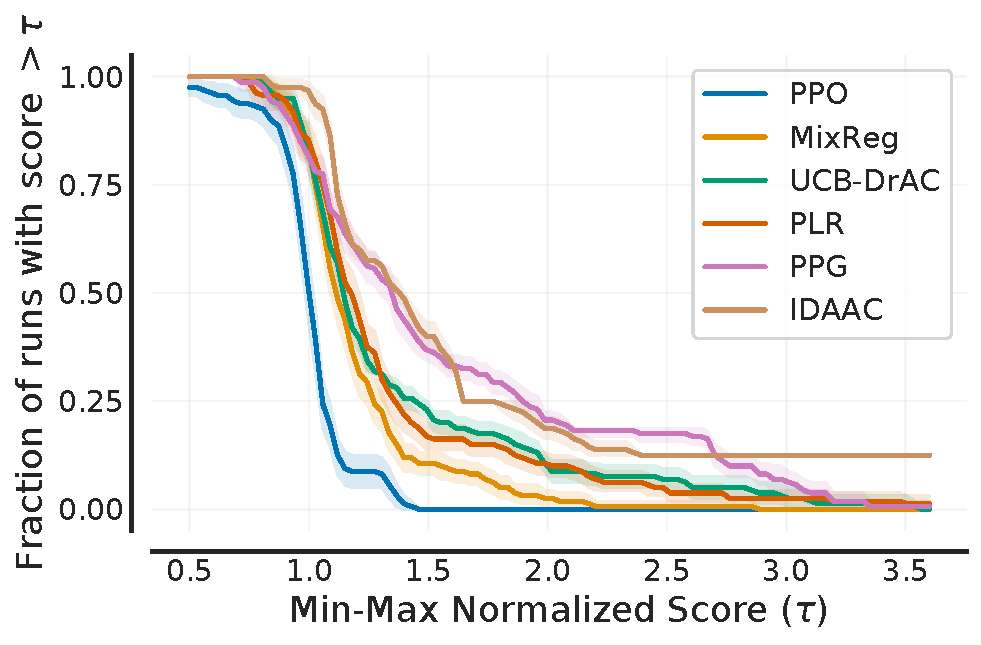
\includegraphics[width=0.43\linewidth]{new_figures/procgen_ppo.pdf}
        % \vspace{-0.5cm}
        % \caption{Score distributions}\label{fig:procgen_profile}
    % \end{subfigure}
    % \begin{subfigure}[c]{0.49\textwidth}
        % \centering
        ~~
        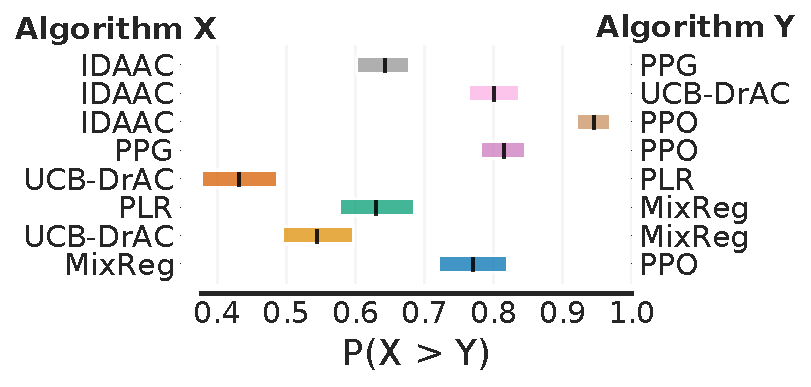
\includegraphics[width=0.47\linewidth]{new_figures/procgen_probability_new.pdf}
        % \caption{Probability of Improvement.}\label{fig:probability_of_improvement}
    % \end{subfigure}
    \vspace{-0.1cm}
    \caption{\textbf{Procgen evaluation} results based on easy mode comparisons~\citep{raileanu2021decoupling} with 16 tasks. \textbf{Left}. Score distributions which compare PPO~\citep{schulman2017proximal}, MixReg~\citep{wang2020improving}, UCB-DrAC~\citep{raileanu2020automatic}, PLR~\citep{jiang2020prioritized}, PPG~\citep{cobbe2020phasic} and IDAAC~\citep{raileanu2021decoupling}. 
    Shaded regions indicate 95\% percentile stratified bootstrap CIs. \textbf{Right}. Each row shows the probability of improvement, with 95\% bootstrap CIs, that the algorithm $X$ on the left outperforms algorithm $Y$ on the right, given that $X$ was claimed to be better than $Y$.
    For all algorithms, results are based on 10 runs per task.
    }\label{fig:procgen}
    \vspace{-0.45cm}
\end{figure}


\textbf{Procgen benchmark}. Procgen~\citep{cobbe2020leveraging} is a popular benchmark, consisting of 16 diverse tasks, for evaluating generalization in RL. 
%While the benchmark paper recommended using min-max normalization, 
Recent papers report mean PPO-normalized scores on this benchmark to emphasize the gains relative to PPO~\citep{schulman2017proximal} as most methods are built on top of it. However, \figref{fig:procgen}~(left) shows that PPO-normalized scores typically have a heavy-tailed distribution making the mean scores highly dependent on performance on a small fraction of tasks. 
Instead, we recommend using normalization based on the estimated minimum and maximum scores on ProcGen~\citep{cobbe2020leveraging} and reporting aggregate metrics based on such scores~(\figref{fig:procgen_agg_appendix}).
% While the benchmark paper recommended using min-max normalization, we instead recommend
% Since min-max normalized scores are typically bounded between 0 and 1~(\figref{fig:procgen_profile}~(right)), we instead recommend  reporting interval estimates aggregate statistics based on them~(\Secref{sec:better_aggregate}).
While publications sometimes make binary claims about whether they improve over prior methods, such improvements are inherently probabilistic. To reveal this discrepancy, we investigate the following
% \begin{wrapfigure}{r}{0.45\linewidth}
%     \centering
%     \vspace{-0.55cm}
%     \includegraphics[width=\linewidth]{figures/procgen_probability.pdf}
%     \vspace{-0.6cm}
%      \caption{\textbf{Probability of Improvement} averaged across all Procgen tasks. Each row shows the probability, with 95\% bootstrap CIs, that the algorithm $X$ on the left outperforms algorithm $Y$ on the right, given that $X$ was claimed to be better than $Y$.}\label{fig:probability_of_improvement}
%     \vspace{-0.55cm}
% \end{wrapfigure}
question: ``What is the probability that an algorithm which claimed improvement over a prior algorithm performs better than it?''~(\figref{fig:procgen}, right). While this probability does not distinguish between two algorithms which uniformly improve on all tasks by 1\% and 100\%, it does highlight how likely an improvement is. For example, there is only a $40-50$\% chance that UCB-DrAC~\citep{raileanu2020automatic} improves upon PLR~\citep{jiang2020prioritized}. We note that a number of improvements reported in the existing literature are only $50-70$\% likely. 